\documentclass{article}
\usepackage{tabularx}
\usepackage{graphicx}
\usepackage{dirtytalk}
\usepackage{pgfplotstable} 
\usepackage{pgfplots}
\usepackage{datatool}
\usepackage{siunitx}
\usepackage[hyphens]{url}
\usepackage{hyperref}
\usepackage{graphicx}
\usepackage{microtype}
\usepackage{float}
\usepackage[style=ieee]{biblatex}
\usepackage{listings}
\usepackage{xcolor}
\usepackage[normalem]{ulem}
\useunder{\uline}{\ul}{}

\addbibresource{main.bib}

\hypersetup{
    colorlinks=true,
    linkcolor=blue,
    filecolor=blue,      
    urlcolor=blue,
    citecolor=blue,
}

\pgfplotsset{compat=1.18}

\title{\textbf{Parallel and Distributed Computing\\DD2443 - Pardis24\\Exercises for Lecture 2}}
\author{Name: Casper Kristiansson}
\date{\today}

\begin{document}

\setlength\parindent{0pt}
\setlength{\parskip}{\bigskipamount}

\maketitle

\section*{Exercise 1}
\subsection*{Question}
\textbf{Consider the class \texttt{VolatileCounters} in Figure 1. The ``volatile'' declaration ensures that variable reads and writes occur in a one-at-a-time sequential order (as one might expect) when accessed by each of the parallel threads. Assume \texttt{actor1} and \texttt{actor2} are invoked to run in parallel.}

\begin{enumerate}
    \item \textbf{What are the relevant events?}
    \item \textbf{Sketch the state machine graph (only parts, it is quite large). Include all events you have identified in 1.}
    \item \textbf{Sketch a few traces of the state machine.}
    \item \textbf{List the relevant intervals for the program.}
    \item \textbf{Which are the possible final values for \texttt{x}? Explain your reasoning very carefully.}
\end{enumerate}

\textbf{Note that this is more subtle than it looks. Are you sure that you have the right solution?}

\subsection*{Answer}
\subsubsection*{1.}
For this program, the relevant events are regarding the reading and writing to the variable x. Since it is declared using volatile to make sure that reading and writing to it happens in sequential order. The actions can be described as:

\begin{itemize}
    \item Read Event: This happens when we want to read the variable \cite{Volatile76:online}. For example, we can assign Read1(x) for actor1 and Read2(x) for actor 2 when reading the variable x.
    \item Write Event: These are the events when we write to the variable x. This can be assigned as Write1(x, newValue) for actor1 and Write2(x, newValue) for actor2.
\end{itemize}


\subsubsection*{2.}

\begin{figure}[h]
    \center
    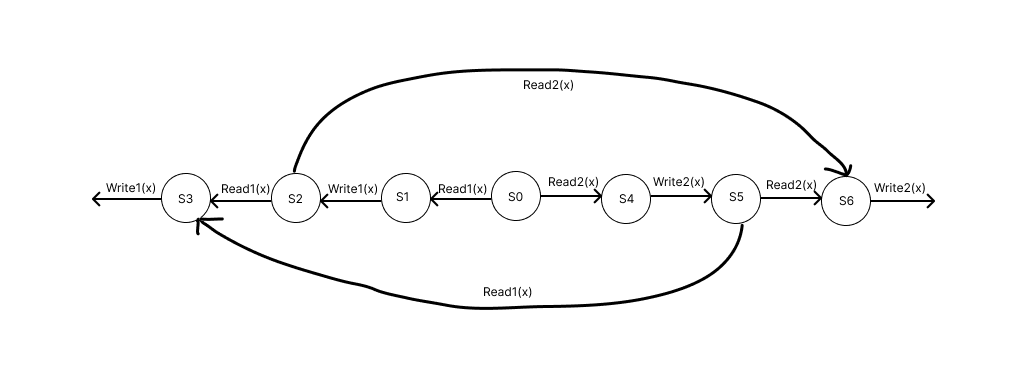
\includegraphics[width=1\textwidth]{LaTex/images/Assignment2.png}
    \caption{State Machine Graph}
    \label{fig:Assignment2}
\end{figure}

In the different states, we have the following:

\begin{enumerate}
    \item State 1: x=0, Read1=false, Read2=false
    \item State 1: x=0, Read1=true, Read2=false
    \item State 2: x=1, Read1=false, Read2=false
    \item State 3: x=1, Read1=true, Read2=false
    \item State 4: x=0, Read1=false, Read2=true
    \item State 5: x=1, Read1=false, Read2=false
    \item State 6: x=1, Read1=false, Read2=true
\end{enumerate}

Note that this is only showing the real beginning of the state machine.


\subsubsection*{3.}
Here are two different traces of how it could look like for the incrementing between the two other actors.

\begin{itemize}
    \item Read1(x=0), Write1(x=1)
    \item Read1(x=1), Write1(x=3)
    \item Read1(x=2), Write1(x=4)
    \item ...
    \item Read2(x=19), Write2(x=20)
\end{itemize}

\begin{itemize}
    \item Read1(x=0), Write1(x=1)
    \item Read2(x=1), Write2(x=2)
    \item Read1(x=3), Write1(x=4)
    \item ...
    \item Read2(x=19), Write2(x=20)
\end{itemize}


\subsubsection*{4.}
There are different types of intervals the program can take. These are the following different intervals that are interesting:

\begin{enumerate}
    \item The interval between actor1 and actor2: It this scenario the read and write will change between actor1 and actor2 after each has finished a sequence of (read-write). This means that first actor1 will increase the counter and than actor2 will increase it etc.
    \item Full increment for actor1: This means that actor1 will finish its incrementing before actor2 starts incrementing.
    \item Full increment for actor2: This means that actor2 will finish its incrementing before actor1 starts incrementing.
\end{enumerate}


\subsubsection*{5.}
With the usage of volatile every read and write of the variable x will be seen as a chunk and lock the variable. This means that if actor1 is in the process of reading/writing to a variable another actor is not able to access it until it gets realsed. Because of the usage of volatile in this situation, the only possible final value of x is that it is 20. It ensures that variable reads and writes occur in a one-at-a-time sequential order.


\section*{Exercise 2}
\subsection*{Question}
\textit{\textbf{HSLS Exercise 2.3 (Flaky Computer Corporation) Use the method presented in class and in the textbook to solve this.}}

\textbf{Programmers at the Flaky Computer Corporation designed the protocol shown in Fig. 2.16 to achieve \textit{n}-thread mutual exclusion. For each question, either sketch a proof or display an execution where it fails.}

\begin{itemize}
    \item \textbf{Does this protocol satisfy mutual exclusion?}
    \item \textbf{Is this protocol starvation-free?}
    \item \textbf{Is this protocol deadlock-free?}
    \item \textbf{Is this protocol livelock-free?}
\end{itemize}

\subsection*{Answer}
\subsubsection*{1.}
Yes, this function with lock and unlock does provide mutual exclusion. This is because when entering the function lock a thread will write to the object its id. It is then only that id will be able to enter the while true loop when busy is false. While all threads will constantly change the variable turn to me there will always only be one that can enter and set busy to true. Doing this allows for mutual exclusion.


\subsubsection*{2.}
No this doesn't provide a starvation-free program. This is because currently, a random thread will be the one setting busy to true. Because with the current scenario, the threads will over and over overwrite the turn variable to me. Meaning if it times it right and the turn is equal to a specific thread and busy becomes false than that thread will enter. If with bad luck this could leave a thread not being able to execute code.


\subsubsection*{3.}
Yes, this program is deadlock-free because it doesn't have a scenario where the current executing thread relies on a thread that might be waiting for its turn. But this will only happen if the critical section doesn't rely on another locking mechanism which in this case it doesn't.


\subsubsection*{4.}
No, with this current type of lock mechanism, there might be a scenario where the threads might constantly change the turn variable to me while the other is trying to check if turn == me. This means that it constantly changes and is busy and its turn is then mismatched leading to that it isn't able to enter its critical zone. This means that the mechanism is not livelock-free.



\section*{Exercise 3}
\subsection*{Question}
\textbf{\textit{HSLS Exercise 2.8 (Fast path lock) Use the method presented in class and in the textbook to solve this.}}

\textbf{In practice, almost all lock acquisitions are uncontended, so the most practical measure of a lock’s performance is the number of steps needed for a thread to acquire a lock when no other thread is concurrently trying to acquire the lock. Scientists at Cantaloupe-Melon University have devised the following “wrapper” for an arbitrary lock, shown in Fig. 2.18. They claim that if the base \texttt{Lock} class provides mutual exclusion and is starvation-free, so does the \texttt{FastPath} lock, but it can be acquired in a constant number of steps in the absence of contention. Sketch an argument why they are right, or give a counterexample.}

\subsection*{Answer}
With this type of lock where we will utilize three different paths right, down, or stop a thread can acquire a thread in a constant number of threads. The protocol works as follows; First, it will check if right is already set to True which it isn't, and will continue to the down path while setting go right to true. This will then in turn if another thread enters the protocol it will go right which often involves that the thread can't acquire the lock right away and needs to wait.

With the usage of a FastPath, it will allow threads to either acquire the lock right away or via the right path. Utilizing this method will mean that the algorithm is both Mutual Exclusion and starvation-free. This is said as long as the Base lock functions correctly.


\newpage
\printbibliography

\end{document}